\section{Preventivo}
Per descrivere come il gruppo \emph{TechSWEave} utilizzerà le risorse a sua disposizione, abbiamo stilatto delle tabelle orarie con la suddivisione dei ruoli, uttilizzando le seguenti sigle:
\begin{itemize}
    \item \textbf{Re: }\emph{Responsabile};
    \item \textbf{Am: }\emph{Amministratore}
    \item \textbf{An: }\emph{Analista};
    \item \textbf{Pt: }\emph{Progettista};
    \item \textbf{Pr: }\emph{Programmatore};
    \item \textbf{Ve: }\emph{Verificatore};
\end{itemize}

\subsection{Fase di Analisi}
    \subsubsection{Prospetto orario}
    In questa fase la distribuzione oraria è la seguente:
    %fare tabella e istogramma 
    %---------------------
    \begin{figure}[!h]
            \caption{Istogramma orari suddivisione dei ruoli}
            \vspace{5px}
            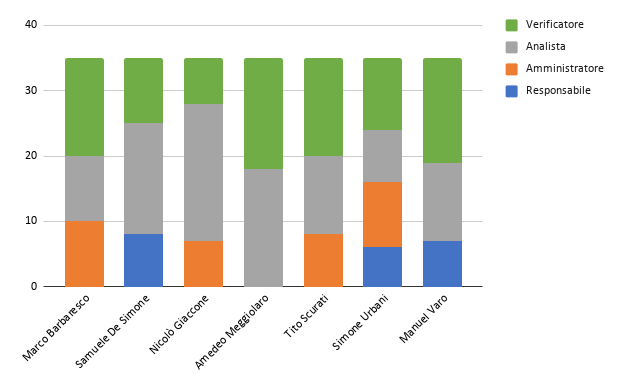
\includegraphics[scale=0.6]{../../../Images/Diagrammi/Istogrammi/ore analisi.png}
            \centering
        \end{figure}
    \subsubsection{Prospetto economico}
    In questa fase i costi da affrontare per ogni ruolo sono i seguenti:
    %fare tabella e istogramma 
    %---------------------

    \begin{figure}[!h]
        \caption{aerogramma ore per ruolo}
        \vspace{5px}
        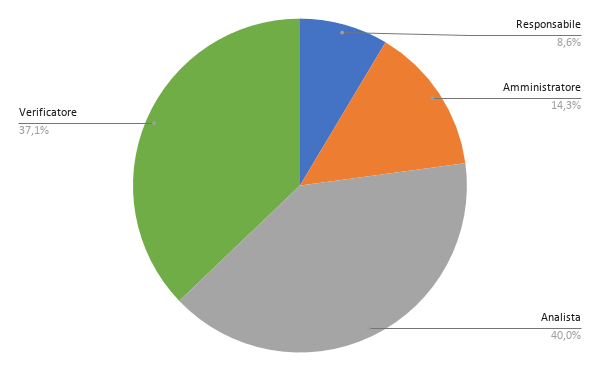
\includegraphics[scale=0.5]{../../../Images/Diagrammi/Diagramma a torta/ore analisi.png}
        \centering
    \end{figure}

    \pagebreak
\subsection{Fase di Consolidamento dei requisiti}
    \subsubsection{Prospetto orario}
    In questa fase la distribuzione oraria è la seguente:
    %fare tabella e istogramma 
    %---------------------
    \begin{figure}[!h]
        \caption{Istogramma orari suddivisione dei ruoli}
        \vspace{5px}
        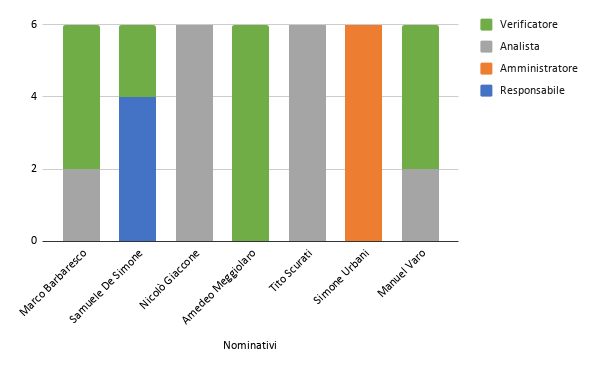
\includegraphics[scale=0.6]{../../../Images/Diagrammi/Istogrammi/ore requisiti.png}
        \centering
    \end{figure}
\subsubsection{Prospetto economico}
In questa fase i costi da affrontare per ogni ruolo sono i seguenti:
%fare tabella e istogramma 
%---------------------

\begin{figure}[!ht]
    \caption{aerogramma ore requisiti per ruolo}
    \vspace{5px}
    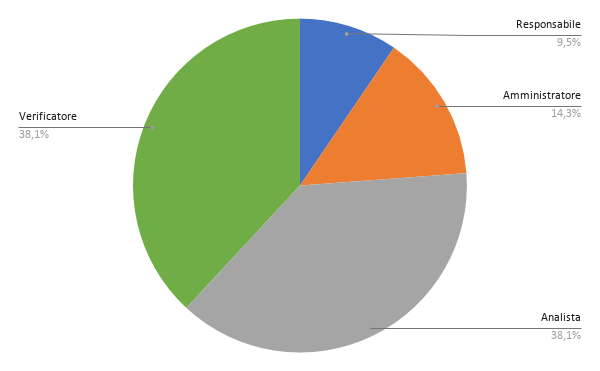
\includegraphics[scale=0.5]{../../../Images/Diagrammi/Diagramma a torta/ore requisiti.png}
    \centering
\end{figure}
\subsection{Fase di Progettazione architetturale}
    \subsubsection{Prospetto orario}
    In questa fase la distribuzione oraria è la seguente:
    %fare tabella e istogramma 
    %---------------------
    \subsubsection{Prospetto economico}
    In questa fase i costi da afforontare per ogni ruolo sono i seguenti:
    %fare tabella e istogramma 
    %---------------------
\subsection{Fase di dettaglio e codifica}
    \subsubsection{Prospetto orario}
    In questa fase la distribuzione oraria è la seguente:
    %fare tabella e istogramma 
    %---------------------
    \subsubsection{Prospetto economico}
    In questa fase i costi da afforontare per ogni ruolo sono i seguenti:
    %fare tabella e istogramma 
    %---------------------    
\subsection{Fase di Validazione e collaudo}
    \subsubsection{Prospetto orario}
    In questa fase la distribuzione oraria è la seguente:
    %fare tabella e istogramma 
    %---------------------
    \subsubsection{Prospetto economico}
    In questa fase i costi da afforontare per ogni ruolo sono i seguenti:
    %fare tabella e istogramma 
    %---------------------    
\subsection{Riepologo}
    \subsubsection{Ore totali}
        \subsubsubsection{Suddivisione lavoro}
        Nella tabella sono riportate il totale delle ore del progetto, sono presenti sia le ore di investimento che quelle rendicontate a carico del commitente:
        %fare tabella e istogramma 
        %---------------------    
        \subsubsubsection{Prospetto economico}
        I costi da affrontare per ogni ruolo sono i seguenti:
        %fare tabella e istogramma 
        %---------------------   
    \subsubsection{Ore rendicontate}
        \subsubsubsection{Suddivisione lavoro}
        Le ore rendicontante sono riportate nella seguente tabella:
        \subsubsubsection{Prospetto economico}
        Il totale rendicontato dei costi da affrontare per ogni ruolo è:
        %mettere tabella 